

\section{Eigenanalysis in R}

The \lstinline!eigen()! function computes the eigenvalues and
eigenvectors of a square matrix.

\begin{lstlisting}
> A <- matrix(c(2,1,2,3),nrow=2)
> A
     [,1] [,2]
[1,]    2    2
[2,]    1    3
> eigen.A <- eigen(A)
> eigen.A
$values
[1] 4 1
$vectors
           [,1]       [,2]
[1,] -0.7071068 -0.8944272
[2,] -0.7071068  0.4472136
> V <- eigen.A$vectors
> D <- diag(eigen.A$values)
> Vinv <- solve(V)
> V %*% D %*% Vinv  # reconstruct our original matrix (see lecture slides)
     [,1] [,2]
[1,]    2    2
[2,]    1    3
> Vinv %*% A %*% V
             [,1] [,2]
[1,] 4.000000e+00    0
[2,] 2.220446e-16    1
> all.equal(Vinv %*% A %*% V, D) # test 'near equality'
[1] TRUE
> V[,1] %*% V[,2] # note that the eigenvectors are NOT orthogonal. Why?
          [,1]
[1,] 0.3162278
> B <- matrix(c(2,2,2,3),nrow=2) # define another tranformation 
> B
     [,1] [,2]
[1,]    2    2
[2,]    2    3
> eigen.B$values
[1] 4.5615528 0.4384472
> eigen.B$vectors
          [,1]       [,2]
[1,] 0.6154122 -0.7882054
[2,] 0.7882054  0.6154122
> Vb <- eigen.B$vectors
> Vb[,1] %*% Vb[,2] # these eigenvectors ARE orthogonal.
     [,1]
[1,]    0
\end{lstlisting}
As we discussed in lecture, the eigenvectors of a square matrix,
$\mathbf{A}$, point in the directions that are unchanged by the
transformation specified by $\mathbf{A}$. The following relationships
relate $\mathbf{A}$ to it's eigenvectors and eigenvalues:

\[\mathbf{V}^{-1}\mathbf{A}\mathbf{V}  =  \mathbf{D} \]

\[\mathbf{A}  =  \mathbf{V}\mathbf{D}\mathbf{V}^{-1}\]

Since $A$ and $B$ represent 2D transformations we can visualize the
effect of these transformations using points in the plane. We'll show
how they distort a set of points that make up a square.

\begin{lstlisting}
# define the corners of a square
> pts <- matrix(c(1,1, 1,-1, -1,-1, -1,1),4,2,byrow=T)
> pts
     [,1] [,2]
[1,]    1    1
[2,]    1   -1
[3,]   -1   -1
[4,]   -1    1
> plot(pts,xlim=c(-6,6),ylim=c(-6,6),asp=1) # plot the corners
> polygon(pts) # draw edges of square
> transA <- A %*% t(pts)
> transA
     [,1] [,2] [,3] [,4]
[1,]    4    0   -4    0
[2,]    4   -2   -4    2
> newA <- t(transA)
> newA
     [,1] [,2]
[1,]    4    4
[2,]    0   -2
[3,]   -4   -4
[4,]    0    2
> points(newA, col='red') # plot the A transformation
> polygon(newA, lty='dashed', border='red') 
> newB <- t(B %*% t(pts)) # do the same for the B transformation
> polygon(newB, lty='dashed', border='blue')  
> points(newB, col='blue')  
> legend("topleft", c("transformation A","transformation B"),
lty=c("dashed","dashed"),col=c("red","blue"))
\end{lstlisting}
The code given above will produce the plot show in the figure below.

\begin{figure}[htbp]
\centering
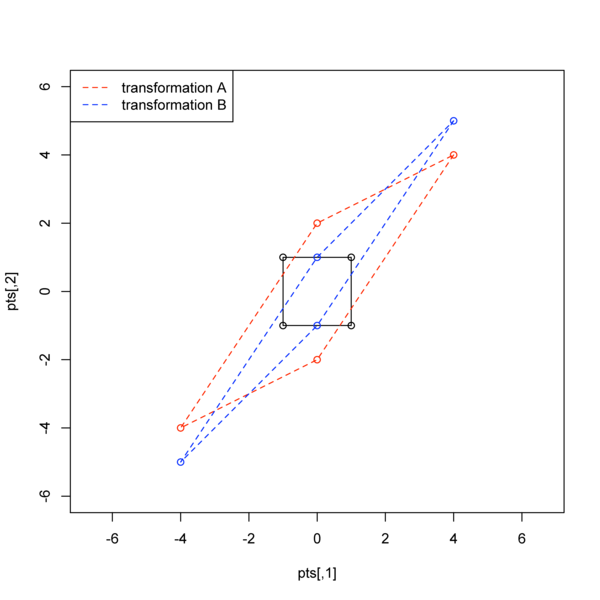
\includegraphics{eigen-transform.png}
\caption{Transformation of a square represented by two matrices, A and
B}
\end{figure}

\begin{quote}
\textbf{Extra Credit}: write R code to reconstruct the plot shown in the
figure below (Fig.~\ref{fig:eigen}) which illustrates the geometry of the eigenvectors for
matrices A and B. Note that the lengths of the eigenvector depictions
are scaled to be proportional to their eigenvalues.

\end{quote}
\begin{figure}[htbp]
\centering
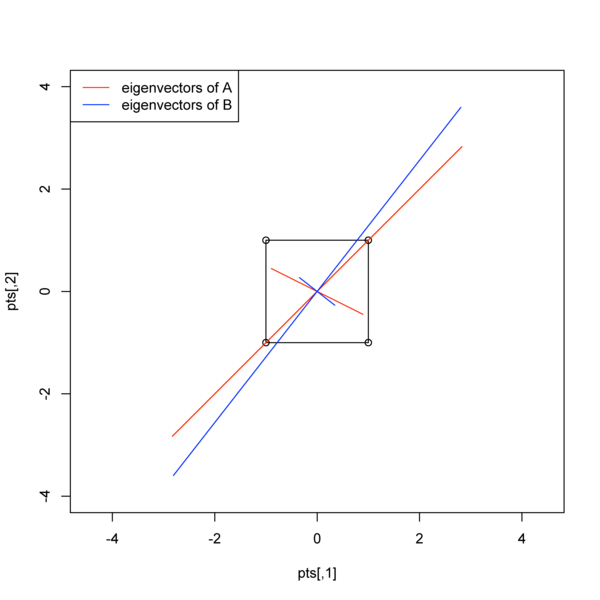
\includegraphics{eigen-ECplot.png}
\caption{Eigenvectors of matrices A and B \label{fig:eigen}}
\end{figure}

\section{Eigenanalysis in Python}

The eigenanalysis functions in Python are found in the
\lstinline!linalg! module in the \lstinline!Numpy! package. These
functions are specified by \lstinline!linalg.eig()! (which returns both
eigenvalues and eigenvectors) and \lstinline!linalg.eigvals()! (which
only returns the eigenvalues).

\begin{lstlisting}
>>> import numpy as np, numpy.linalg as la
>>> A = np.array([[2,2],[1,3]],np.float)
>>> A
array([[ 2.,  2.],
       [ 1.,  3.]])
>>> evals, evecs = la.eig(A)
>>> evals
array([ 1.,  4.])
>>> evecs
array([[-0.89442719, -0.70710678],
       [ 0.4472136 , -0.70710678]])
\end{lstlisting}
Note that (somewhat inconveniently) the \lstinline!eig()! function does
not necessarily return the eigenvalues and eigenvectors in sorted
fashion. The Numpy documentation states that the normalized eigenvector
corresponding to the eigenvalue \lstinline!w[i]! is the column
\lstinline!v[:,i]!. Also note that both the R \lstinline!eigen()!
function and the Numpy \lstinline!eig()! function return normalized
eigenvectors (i.e.~each eigenvector has length 1).

We can get sort the eigenvectors by their eigenvalues as so:

\begin{lstlisting}
>>> colorder = list(np.argsort(evals)) # get back argsort as a list
>>> colorder
[0, 1]
>>> colorder.reverse() # need to reverse the column order because want from large to small
>>> colorder
[1, 0]
>>> srtevals = np.take(evals, colorder) #see the Numpy docs on take()
>>> srtevals
array([ 4.,  1.])
>>> srtevecs = np.take(evecs, colorder,axis=1) # sort columns
>>> srtevecs
array([[-0.70710678, -0.89442719],
       [-0.70710678,  0.4472136 ]])
>>> V = srtevecs
>>> Vinv = la.inv(srtevecs)
>>> D = np.diag(srtevals)
>>> np.dot(V, np.dot(D, Vinv))
array([[ 2.,  2.],
       [ 1.,  3.]])
>>> Arecon = np.dot(V, np.dot(D, Vinv))
>>> Arecon == A
array([[ True,  True],
       [ True, False]], dtype=bool)
>>> np.allclose(Arecon, A)  # like R's all.equal()
True     
\end{lstlisting}
See the Numpy docs for more information on the \lstinline!argsort()!
(\href{http://docs.scipy.org/doc/numpy/reference/routines.sort.html}{Numpy:
Sorting and searching}), \lstinline!take()!
((\href{http://docs.scipy.org/doc/numpy/reference/routines.indexing.html}{Numpy:
Indexing Routines}), and \lstinline!allclose()!
(\href{http://docs.scipy.org/doc/numpy/reference/routines.logic.html}{Numpy:
Logic functions}).

\begin{quote}
\textbf{Assignment 1}: Write a Python function that takes as input a
square matrix, and returns a vector of sorted eigenvalues (sorted from
largest to smallest) and the corresponding matrix of eigenvectors sorted
according to their corresponding eigenvalues.

\end{quote}
\section{Principal Components Analysis in R}

There are two functions in R for carrying out PCA -
\lstinline!princomp()! and \lstinline!prcomp()!. The
\lstinline!princomp()! function uses the \lstinline!eigen()! function to
carry out the analysis on the covariance matrix or correlation matrix,
while \lstinline!prcomp()! carries out an equivalent analysis, starting
from a data matrix, using a technique called singular value
decomposition (SVD). The SVD routine has greater numerical accuracy so
it should generally be preferred but we'll delay it's use until next
week when we introduce the mathematics behind SVD. The
\lstinline!princomp()! function is also useful when you don't have
access to the original data, but you do have a covariance or correlation
matrix (a frequent situation when re-analyzing data from the
literature). By default the \lstinline!princomp()! function carries out
PCA on the covariance matrix of the data. If you wish to carry out PCA
using the correlation matrix specify the argument \lstinline!cor=T!.

To demonstrate PCA we'll use Anderson's Iris data set.

\begin{lstlisting}
> names(iris)
[1] "Sepal.Length" "Sepal.Width"  "Petal.Length" "Petal.Width"  "Species"     
> iris
    Sepal.Length Sepal.Width Petal.Length Petal.Width    Species
1            5.1         3.5          1.4         0.2     setosa
2            4.9         3.0          1.4         0.2     setosa
3            4.7         3.2          1.3         0.2     setosa    
.. output truncated ..
> summary(iris) # notice that  Petal.Width is
        # about an order of magnitude smaller than the other variables.
        # We should therefore consider doing the PCA on the correlation
        # matrix rather than the cov matrix. We'll try both
> setosa <- subset(iris, Species=='setosa', select=-Species)        
> pca.setosa <- princomp(setosa)
> summary(pca.setosa)
Importance of components:
                          Comp.1    Comp.2    Comp.3     Comp.4
Standard deviation     0.4813799 0.1902114 0.1620508 0.09408823
Proportion of Variance 0.7647237 0.1193992 0.0866625 0.02921456
Cumulative Proportion  0.7647237 0.8841229 0.9707854 1.00000000
> plot(pca.setosa) # plots histogram plot of eigenvalues
> plot(pca.setosa$scores)  # in space of PC1 and PC2
> plot(pca.setosa$scores, asp=1)  # compare to the previous plot     
> plot(pca.setosa$scores[,1],pca.setosa$scores[,3], asp=1) # PC1 and PC3
> pca.setosa$loadings

Loadings:
             Comp.1 Comp.2 Comp.3 Comp.4
Sepal.Length -0.669 -0.598  0.440       
Sepal.Width  -0.734  0.621 -0.275       
Petal.Length        -0.490 -0.832 -0.240
Petal.Width         -0.131 -0.195  0.970

               Comp.1 Comp.2 Comp.3 Comp.4
SS loadings      1.00   1.00   1.00   1.00
Proportion Var   0.25   0.25   0.25   0.25
Cumulative Var   0.25   0.50   0.75   1.00

# now do the PCA based on the correlation matrix
> pca.setosa.cor <- princomp(setosa,cor=T)
> summary(pca.setosa.cor)
Importance of components:
                          Comp.1    Comp.2    Comp.3     Comp.4
Standard deviation     1.4347614 1.0110283 0.8172027 0.50145917
Proportion of Variance 0.5146351 0.2555446 0.1669551 0.06286532
Cumulative Proportion  0.5146351 0.7701796 0.9371347 1.00000000
> pca.setosa.cor$loadings

Loadings:
             Comp.1 Comp.2 Comp.3 Comp.4
Sepal.Length  0.604  0.335         0.720
Sepal.Width   0.576  0.441        -0.689
Petal.Length  0.375 -0.627 -0.677       
Petal.Width   0.403 -0.548  0.733       

               Comp.1 Comp.2 Comp.3 Comp.4
SS loadings      1.00   1.00   1.00   1.00
Proportion Var   0.25   0.25   0.25   0.25
Cumulative Var   0.25   0.50   0.75   1.00
> plot(pca.setosa.cor)
> plot(pca.setosa.cor$scores,asp=1)
\end{lstlisting}
\begin{quote}
\textbf{Assignment 2}: Do a PCA analysis on the iris data set with all
three species pooled together. Generate a plot showing the projection of
the specimens on the first two PC axes as shown in the figure below.
Represent the specimens from a given species with different colors. Make
sure you include a legend for your plot.

\end{quote}
\begin{quote}
Apply PCA (on the covariances) to the \lstinline!yeast-subnetwork! data
set from week three. Now do the same analysis based on PCA of the
correlation matrix. How does your interpretation of the data change?

\end{quote}
\begin{figure}[htbp]
\centering
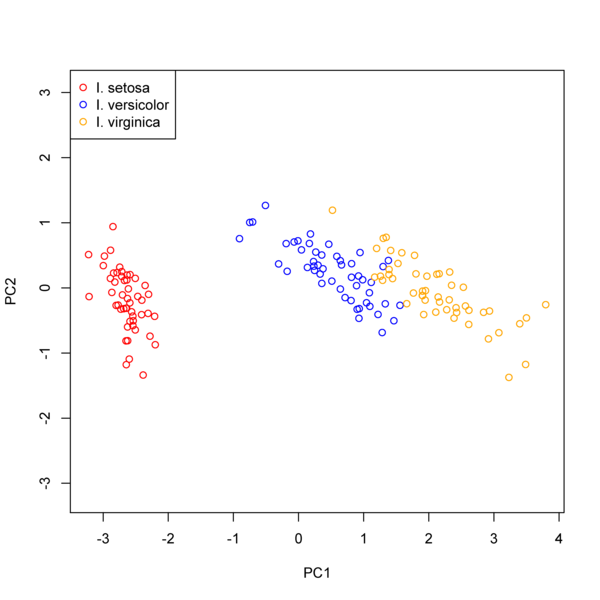
\includegraphics{iris-all-pca.png}
\caption{PCA of the iris data set. One of your assignments is to
reconstruct this figure on your own.}
\end{figure}

\section{Principal Components Analysis in Python}

There are no built-in functions for carrying out PCA in Python. Luckily
you have all the tools you need at your disposal to write your own PCA
module.

Note that when performing PCA on a correlation matrix, to get the proper
PC scores you need to use mean centered and standardized variates.

Here's an example:

\begin{lstlisting}
>>> import numpy as np, numpy.linalg as la
>>> turt = np.loadtxt('turtles.txt',skiprows=1,usecols=(1,2,3)) # see the Numpy docs
>>> turt.shape
(48, 3)
>>> import pylab # convenient interface to Matplotlib
>>> pylab.scatter(turt[:,0], turt[:,1])
<matplotlib.collections.CircleCollection object at 0x2502630>
>>> pylab.show()
>>> pylab.scatter(turt[:,0], turt[:,2])
<matplotlib.collections.CircleCollection object at 0x66d4a30>
>>> pylab.scatter(turt[:,1], turt[:,2])
<matplotlib.collections.CircleCollection object at 0x63296b0>
>>> tmean = np.mean(turt,axis=0) # get the column means
>>> tmean
array([ 124.6875    ,   95.4375    ,   46.33333333])
>>> deviates = turt - tmean # this mean centers each observation
>>> stdized = deviates/np.std(deviates,axis=0) # standardize variates
>>> pylab.scatter(stdized[:,0],stdized[:,1],color='red') # plot the standardized observations
>>> tcor = np.corrcoef(turt,rowvar=False)
>>> tcor
array([[ 1.        ,  0.97831162,  0.96469455],
       [ 0.97831162,  1.        ,  0.96057053],
       [ 0.96469455,  0.96057053,  1.        ]])
>>> u,v = la.eig(tcor)
>>> u # the eigenvalues
array([ 2.93573765,  0.02141848,  0.04284387])
>>> v  
array([[-0.57879812, -0.74789704, -0.32502731],
       [-0.57798399,  0.65741263, -0.48346989],
       [-0.57526276,  0.09197088,  0.81278171]])
>>> colsort = np.argsort(u)[::-1] # fancy way  to do the 
                  # argsort and reversing to sort index in one call
>>> colsort
array([0, 2, 1])
>>> usort = np.take(u,colsort)
>>> vsort = np.take(v,colsort,axis=1)
>>> usort
array([ 2.93573765,  0.04284387,  0.02141848])
>>> vsort # the PC coefficents are the normalized eigenvectors
array([[-0.57879812, -0.32502731, -0.74789704],
       [-0.57798399, -0.48346989,  0.65741263],
       [-0.57526276,  0.81278171,  0.09197088]])
>>> L = np.diag(usort**0.5) # mtx with sqrt of eigenvalues on diagonal
>>> L
array([[ 1.71339944,  0.        ,  0.        ],
       [ 0.        ,  0.2069876 ,  0.        ],
       [ 0.        ,  0.        ,  0.14635054]])
>>> f=np.dot(vsort,L) # "factor loadings" -- gives corr. btw original vars and PC axes
>>> f
array([[-0.99171237, -0.06727662, -0.10945514],
       [-0.99031745, -0.10007227,  0.09621269],
       [-0.98565489,  0.16823574,  0.01345999]])
>>> scores = np.dot(stdized,vsort)
>>> scores[:5]  # compare to the values you got in R
array([[ 2.00466025,  0.16892135,  0.13583391],
       [ 1.72362844, -0.02689852,  0.10856089],
       [ 1.35439901,  0.2874806 ,  0.25768234],
       [ 1.43581697,  0.05967203,  0.16172995],
       [ 0.95235368,  0.30990249,  0.16324351]])
>>> pylab.scatter(scores[:,0],scores[:,1]) # don't close the plot 
                                        # or else the next line won't work
<matplotlib.collections.CircleCollection object at 0x66d5f50>
>>> pylab.axes().set_aspect(1) # equivalent of the asp=1 argument in R
>>> pylab.xlim(-5,3)  # to make the plot limits more like those we saw in R
(-5, 3)
>>> pylab.ylim(-3,3)
(-3, 3)
\end{lstlisting}
\begin{quote}
\textbf{Assignment 3}: Write a Python function that takes as it's input
an $n \times p$ data matrix and returns the following four objects
(\emph{in this order}):

\begin{enumerate}[1.]
\item
  A vector of the \textbf{eigenvalues of the correlation matrix} sorted
  from largest to smallest
\item
  A corresponding matrix of \textbf{eigenvectors of the correlation
  matrix} sorted relative to their eigenvalues
\item
  The \textbf{principal component scores} for the dataset
\item
  An array giving the percentage of variation explained by each
  principal component.
\end{enumerate}
Apply this to the \lstinline!yeast-subnetwork! data set and check your
answers against the R implementation.

\end{quote}
